\chapter{Required Properties of E2E Systems\ifdraft{ (Dan) (35\%)}{}}
\label{chapter:required_properties}

To describe the properties that E2E election systems must fulfill we
must start from a technical definition of the term ``E2E'', which was
defined informally in \autoref{chapter:e2e_viv_explained}. From there
we can proceed to a formal protocol description of an ideal E2E
system, and finally to a set of formal requirements that must be met
by any real-world implementation of such a system.\tododmz{I don't
  like ``chapter roadmap'' text as a general rule, so I'll do better
  at some point}

\section{Technical Definition of E2E}

\tododmz{This section will essentially be a restatement of section ``IV,
  VIV, E2E'' in \autoref{chapter:e2e_viv_explained}, but more
  technical in nature.}

\section{Ideal Functionality of an E2E System---$\fete$}
\tododmz{I think this may want to be the \emph{last} section of the
  chapter, leading into the crypto specification, which can then refer
  to it. Either that, or it should actually be moved into the crypto
  specification chapter...}
The basic protocol followed by any system implementing E2E verifiable
elections can be characterized by an \emph{ideal functionality}. This
ideal functionality, called $\fete$ and presented in
\autoref{fig:required_properties:fete}, recognizes and interacts with
the election authority $\EA$, the set of eligible voters
$V_1,\ldots, V_n$ and the auditor $\AU$.  These are ``ideal-world''
entities; a ``real-world'' implementation of $\fete$ may involve more
parties that will enable the implementation to realize the ideal
functionality.

$\fete$ accepts a number of commands from the election authority
$\EA$, the voters and the auditors. At the same time it informs the
(ideal world) adversary of certain actions that take place and is
influenced by the adversary to perform certain actions. The ideal
functionality keeps track of which parties are corrupted and may act
according to their corruption status.

$\fete$ has two parameters:

\begin{enumerate}
\item A function $f: (X\cup \{\bot\})^n\rightarrow E$ that defines the
  election function, where $X$ defines the set of all possible ways
  for an individual voter to vote and $E$ is the set of all possible
  election results. The notation $X^n$ denotes all possible strings of
  length $n$ over the alphabet $X$. The symbol $\bot$ stands for
  ``undefined.''  The election function $f$ is invariant with respect
  to $\bot$, i.e., $f(\bot, x) = f(x)$ for all $x$.  
\item A relation $Q$ that defines the level of sensitivity to
  manipulation permitted by $\fete$. In particular, for two possible
  election results $T$ and $T'$ we say that $Q(T,T')$ holds if and
  only if $T'$ is sufficiently close to $T$. For the most strict
  version of $\fete$ we define $Q$ to be the equality relation over
  $E$ (that is, $Q(T,T')$ holds if and only if $T=T'$). 
\end{enumerate}

\begin{figure}[t]
\begin{center}
\fbox{
\begin{minipage}[h]{6in}
\begin{center}
\textbf{Functionality $\fete^{f, Q}$}
\end{center}
\vspace{1.5ex}
  The functionality recognizes and interacts with the following
  parties: (i) the election authority $\EA$; (ii) the eligible voters
  $\mc{V}= \{V_1,\ldots, V_n\}$; (iii) the auditor $\AU$; and (iv) the
  adversary $\mc{A}$.  It is parameterized by the relation $Q$ over
  $E$ and the election function $f:(X\cup\{\bot\})^n \rightarrow E$.
\vspace{1.5ex}
\begin{itemize}
\item Upon receiving an input $(\Create, sid, B)$ from the $\EA$,
  record the tuple $(sid, B)$ such that $sid$ is the election
  identifier and $B$ is a string defining the ballot of the election.
  Send $(\Create, sid, B)$ to the adversary $\mc{A}$.

\item Upon receiving an input $(\Deliver, sid)$ from $\EA$, deliver
  $(B, s_i)$ to each voter $V_i$, where $s_i$ is some voter-specific
  information that is provided by the adversary $\mc{A}$.\footnote{In
    some systems, voters may request this information actively; hence,
    $\fete$ will be passive and will not deliver the ballots.  In such
    cases the adversary will adaptively provide the $s_i$ values.}

\item Upon receiving an input $(\Vote, sid, a)$ from $V_i$, select a
  unique identifier $vid$ and record the tuple $(vid, a)$ provided
  $a\in X$.  If $\EA$ is honest, send $(\Vote,sid, vid)$ to the
  adversary $\mc{A}$; if $\EA$ is corrupted, send
  $(\Vote, sid, vid, V_i, a)$ to $\mc{A}$.\footnote{In some systems
    the voter identity $V_i$ can be leaked to the adversary during
    ballot casting.}

\item Upon receiving $(\RecordVote, sid, vid, b)$ from $\mc{A}$,
  verify that a tuple $(vid, a)$ has been previously recorded and then
  record the tuple $(V_i, a, b)$ provided that (i) $V_i$ is a voter
  that has not previously been assigned a vote,\footnote{In some
    systems the voter is allowed to change his/her mind and hence vote
    multiple times.} (ii) the value $a$ is a valid choice consistent
  with the ballot description $B$, and (iii) the value $b$ is unique
  amongst received $\RecordVote$ messages.  Finally, return
  $(\Receipt, b)$ to $V_i$.

\item Upon receiving an input $(\Tally, sid)$ from the $\EA$, collect
  all recorded inputs $\{(V_j, a_j, b_j)\}_{j\in \tilde{\mc{V}}}$,
  where $\tilde{\mc{V}}$ is the set of voters that voted successfully,
  and set $a_j = \bot$ for all $j\not\in \tilde{\mc{V}}$.  Compute
  $T =f(\langle a_{1}, \ldots, a_n \rangle )$ and return $(\Tally, T)$
  to $\mc{A}$.

\item Upon receiving $(\RecordTally, sid, \mc{M}, \hat{T})$ from
  $\mc{A}$, where $\mc{M}$ can be parsed as a polynomial-size circuit,
  set $\langle a'_{1}, \ldots, a'_n \rangle = \mc{M}(a_1,\ldots,a_n)$
  and if $\exists j: (a'_j \neq a_j)$ and $\EA$ is honest then ignore
  the message. In any other case, record $(\Result, T', \hat{T})$ and
  $\langle a'_{1}, \ldots, a'_n \rangle$, where $T'$ is the election
  result calculated as
  $T' = f(\langle a'_{1}, \ldots, a'_n \rangle )$.

\item Upon receiving $(\ReadTally, sid)$ from any party, 
return $(\Result, \hat{T}, Q(\hat{T},T'))$.

\item Upon receiving $(\Audit, b)$ from  from any party, 
recover the triple $(V_j, a_j,b_j)$ such that $b_j = b$ and return 1 if and only 
if $(a_j' = a_j)$ and 0 otherwise.
\end{itemize}
\end{minipage}
}
\end{center}
\caption{The ideal functionality $\fete^{f,Q}$.}
\label{fig:required_properties:fete}
\end{figure}

The ideal functionality $\fete^{f,Q}$ captures the following set of
security characteristics:

\begin{itemize}
\item Provided the $\EA$ is not corrupted, the adversary is incapable
  of extracting the voters' selections.

\item Provided the $\EA$ is not corrupted, all votes are recorded and
  tallied according to the election function $f(\cdot)$.

\item Even if the $\EA$ is corrupted, a set of well defined votes are
  assigned to the voters of the election (however, such votes may
  deviate from the original voters' intent). The votes cannot be
  manipulated when the $\EA$ is honest.

\item Even if the $\EA$ is corrupted, the functionality consistently
  returns the same tally result to all parties that request
  it. Furthermore, the functionality always tests the reported tally
  according to the predicate $Q$ and reports the outcome, hence any
  substantial (according to $Q$) deviation from the recorded tally
  will be detectable by all honest parties.

\item The functionality preserves voter intent and, in case of vote
  manipulation, the voter or an auditor can use the unique receipts
  provided in the completion of ballot-casting to test whether voter
  intent was manipulated by a corrupt $\EA$. Any party may use those
  receipts, hence verification is ``delegatable.''
\end{itemize}

Consider now a protocol $\pi$ that implements syntactically the ideal
functionality $\fete$ (i.e., has the same I/O characteristics as
$\fete$). Following standard notation and terminology we have the
following:

\begin{definition}
  Let $f$ be an election function and $Q$ a predicate over the
  election results.  The protocol $\pi$ implements $\fete^{f,Q}$
  provided that, for all adversaries $\mc{A}$, there is a simulator
  $\mc{S}$ so that for all environments $\mc{Z}$ it holds that
\[ \Exec_{\pi, \mc{A}, \mc{Z}} \approx
\Exec^{\fete^{f,Q}}_{\mc{S},\mc{Z}}  \ \ .\]
\end{definition}

Note that the protocols that will be considered in practice may
utilize simpler ideal functionalities. In such cases, the protocol
$\pi$ implements $\fete$ conditional on the existence and availability
of these other functionalities. Such functionalities include
``authenticated channels'', a ``write-only bulletin board'', etc.

\paragraph{Party corruption.} As stated, the ideal functionality
$\fete$ enables the adversary $\mc{A}$ to corrupt parties by issuing
special $(\Corrupt, P)$ messages.  Given such a message, the ideal
functionality $\fete$ will divulge to the adversary the complete I/O
transcript from the interface between $\fete$ and $P$. We distinguish
between static and adaptive corruptions. In the case of static
corruptions all messages $(\Corrupt,P)$ are delivered at the onset of
the execution, while for adaptive corruptions they can be delivered at
any time.  For brevity we do not explicitly include the actions taken
for $\Corrupt$ messages in the description of the functionality.

In the real world, the corruption of an entity expresses an action
taken by the adversary that results in the complete control of the
entity's computing environment. A corrupted voter, specifically, loses
privacy completely and the adversary may take any action on her
behalf. For example, if corruption of a voter happens prior to ballot
casting the adversary may vote on her behalf, while if corruption of a
voter happens after ballot casting the adversary will learn her
choice. If the adversary corrupts the $\EA$, it may try to manipulate
some voters' ballots however to the extent permitted by $\fete$ (no
matter how many parties are corrupted, $\fete$ always has the ``upper
hand'').

\subsection{Claims Regarding $\fete$}

\begin{claim}
  Assuming the $\EA$ is not corrupted, the ideal functionality
  $\fete^{f,Q}$ leaks no information about how honest voters vote,
  except for information that is revealed from the partial tally of
  the votes of the honest voters (according to $f$).
\end{claim}

\begin{claim}
  The adversary may delay the recording of an honest voter's ballot,
  however when it is recorded the voter obtains a receipt that enables
  her to verify that her vote has been properly recorded and tallied.
\end{claim}

\begin{claim}
  The receipt each voter obtains after her vote is recorded is unique;
  assuming the $\EA$ is honest, each receipt is independent of the
  voter's choice and hence can safely be passed to, e.g., a third
  party auditor $\AU$.
\end{claim}

\begin{claim}
  When the $\EA$ is corrupted it is possible for the adversary to
  manipulate all the votes (via computational manipulation
  $\mc{M}(a_1,\ldots, a_n) = (a_1', \ldots, a'_n)$) and even provide
  an incorrect tally $\hat{T}$; nevertheless, the ideal functionality
  ensures that honest parties are notified about whether the reported
  tally $\hat{T}$ and the recorded tally $T'$ satisfy the relation
  $Q$, i.e., it returns $Q(T',\hat{T})$.
\end{claim}

\subsection{Security Properties Not Captured by $\fete$}

We have intentionally omitted a number of security aspects from this
specification of the ideal end-to-end functionality $\fete$:

\begin{itemize}
\item \textbf{Denial of service attacks.} The ideal functionality as
  written enables the adversary to prevent voters from completing the
  ballot-casting protocol and prevent the tally from becoming
  available. From a definitional point of view, expressing the
  mitigation of such attacks is feasible by assuming certain qualities
  of the underlying communication and message passing mechanisms
  employed in the implementation. One way to extend the functionality
  to capture such mitigation is to oblige the adversary to deliver the
  $(\RecordVote)$ and $(\RecordTally)$ messages by certain
  deadlines. In order to do this formally, a notion of time would have
  to be introduced in the model, for example by introducing a global
  clock functionality.

\item \textbf{Coercion via corrupting voters.} Even though $\fete$
  does not permit coercion via the receipts it provides, the adversary
  may still achieve coercion by corrupting a voter (e.g., hacking into
  the voter's computer). If this happens after the ballot-casting
  protocol, $\fete$ reveals the choice of the voter and hence the
  voter may be vulnerable to coercion.  Addressing this in the model
  is feasible by further restricting the information that is divulged
  when voter corruption takes place. Various intermediate levels of
  corruption may be considered, e.g., is the voter capable of erasing
  some information? rewriting some information? etc.

\item \textbf{Sybil attacks.} The set of voters $V_1,\ldots,V_n$ is
  predetermined and integrated into the functionality $\fete$. Hence,
  the adversary cannot manipulate the list of voters.  It follows that
  $\fete$ is applicable to the setting where the list of voters is
  predetermined, assumed to be public, and immune to tampering by the
  adversary. 
\end{itemize}

\section{Formal Requirements for E2E VIV Systems}

The requirements for E2E VIV systems can be broadly divided into two
types: technical and non-functional\todokiniry{Should this be
  ``non-technical''? Or alternatively, ``functional and
  non-functional?''}. Technical requirements are those that can be
directly addressed by the design and implementation of the system,
such as authentication requirements for voters and election
officials. Non-functional requirements are those that are imposed
externally to the system or those where the system depends on external
behaviors outside its control, such as specific election certification
guidelines and operational
procedures. \autoref{fig:e2eviv_requirements_hierarchy} is a
high-level overview of the various requirement categories.

\begin{figure}
\begin{center}
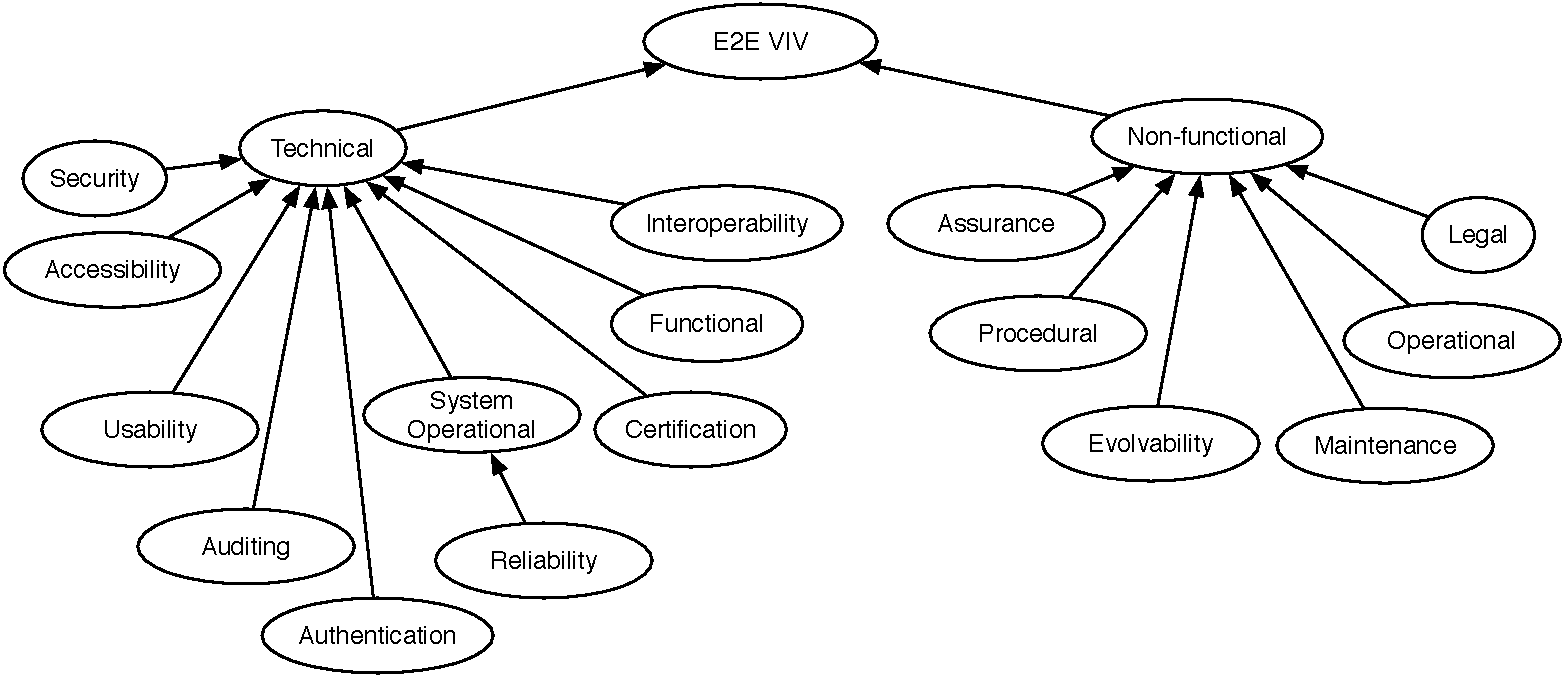
\includegraphics[width=6in]{required_properties_resources/hierarchy}
\end{center}
\caption{The hierarchy of requirements for E2E VIV systems.}
\label{fig:e2eviv_requirements_hierarchy}
\end{figure}

We briefly describe each of these requirement categories and summarize
the requirements therein; \autoref{appendix:bon_requirements} is a
complete listing of the requirements expressed in the Business Object
Notation.

\subsection{Technical Requirements}
There are ten categories of technical requirements for E2E VIV
systems: functional, accessibility, usability, security,
authentication, auditing, system operational, reliability,
certification, and interoperability.

\subsubsection{Functional} 
\lipsum[2]
\subsubsection{Accessibility}
\lipsum[3]
\subsubsection{Usability}
\lipsum[4]
\subsubsection{Security}
\lipsum[5]
\subsubsection{Authentication}
\lipsum[6]
\subsubsection{Auditing}
\lipsum[7]
\subsubsection{System Operational}
\lipsum[8]
\subsubsection{Reliability}
\lipsum[9]
\subsubsection{Certification}
\lipsum[10]
\subsubsection{Interoperability}
\lipsum[11]

\subsection{Non-functional Requirements}
There are six categories of non-functional requirements for E2E VIV
systems: operational, procedural, legal, assurance, maintenance, and
evolvability.

\subsubsection{Operational}
\lipsum[13]

\subsubsection{Procedural}
\lipsum[14]

\subsubsection{Legal}
\lipsum[15]

\subsubsection{Assurance}
\lipsum[16]

\subsubsection{Maintenance}
\lipsum[17]

\subsubsection{Evolvability}
\lipsum[18]
